\section{Computational Implementation}
\subsection[Overview]{Gibbs Energy Minimiser - Overview}

\frame{
	\frametitle{Computational Structure}
	\begin{figure}[htbp]
		\begin{center}
		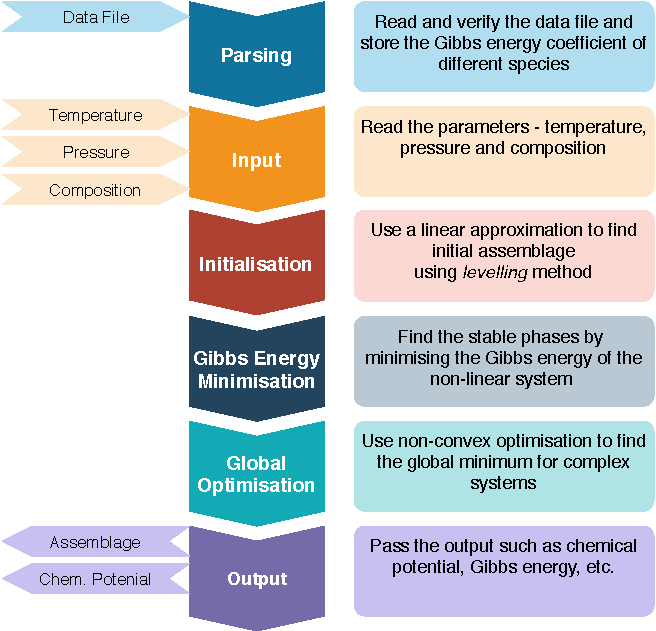
\includegraphics[height=0.65\paperheight]{Figures/YJ_structure.pdf}
		\end{center}
	\end{figure}
}

\subsection{Gibbs Energy Minimiser}
    \frame{
    \frametitle{Parsing}
         \only<1-3>{
             \begin{itemize}
                 \item<1-> The data files are created using the well known Calphad method and can be available in different formats.
                 \item<2-> Most commonly used formats are ThermoCalc (*.tdb) and ChemSage (*.dat).
                 \item<3-> Yellowjacket uses ChemSage (*.dat) format datafiles, which can be generated by the commercial software FactSage.
             \end{itemize}
             }
             \only<4>{\begin{figure}
                 \centering
                 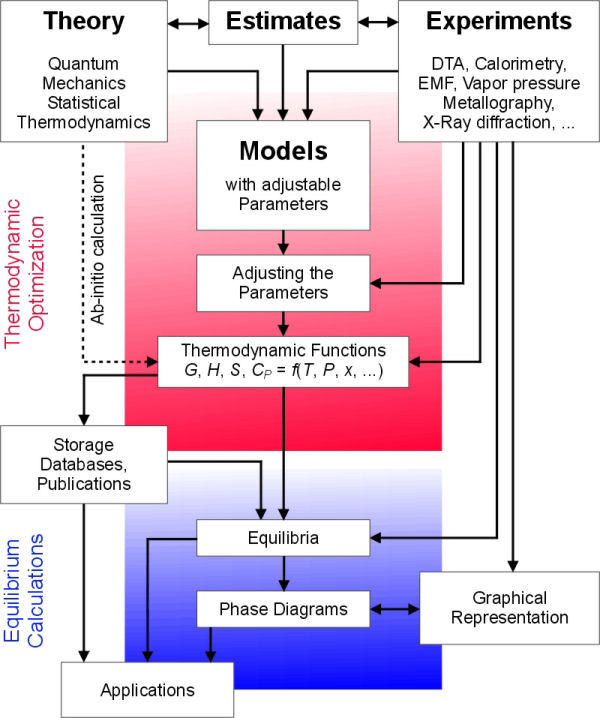
\includegraphics[height=0.75\paperheight]{Figures/Calphad_method.jpg}
             \end{figure}}
  }
    
      \frame{
    \frametitle{Input}
             \begin{itemize}
                 \item Temperature, pressure and composition are required at each time step and for each mesh element.
                 \item At each time step MOOSE can provide these inputs to Yellowjacket.
             \end{itemize}
    }
    

    \frame{
    \frametitle{Initialisation}
             \begin{itemize}
                 \item<1-> Gibbs energy minimisers require an initial estimate of molar quantities of species and phases.
                 \item<2-> \textit{Levelling} is an estimating process developed by Eriksson and Thompson (1989).
                 \item<3-> Levelling converts the non-linear optimisation problem into a linear optimisation problem by treating all species and phases as pure separate phases.
                 \item<4->The number of iterations required to achieve convergence does not increase rapidly with the number of system components.
             \end{itemize}
    }
    
      \frame{
    \frametitle{Initialisation}
         \begin{figure}
             \centering
             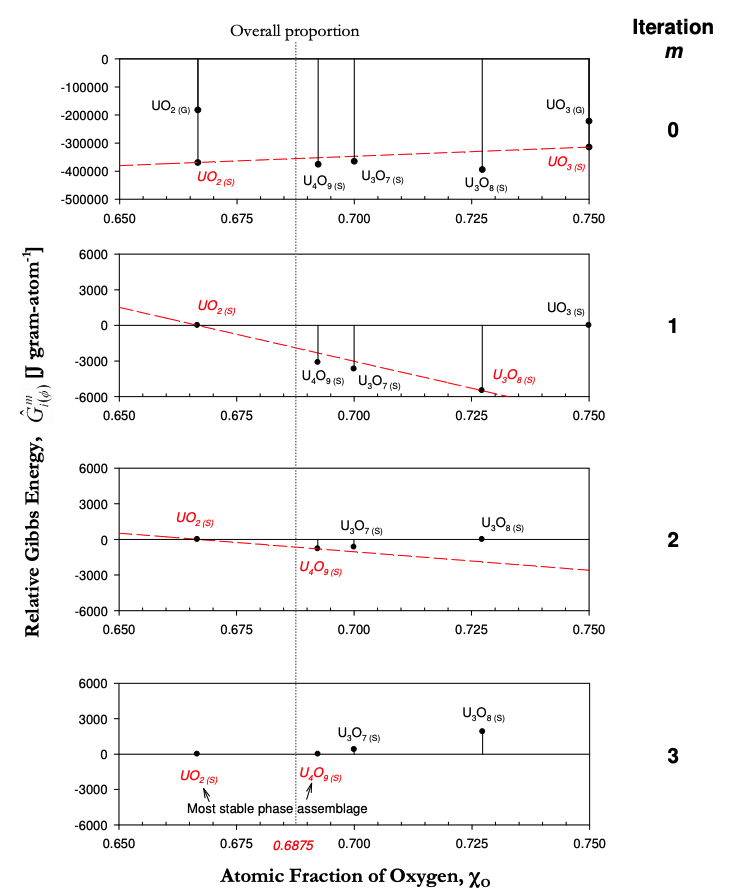
\includegraphics[height=0.75\paperheight]{Figures/Levelling_illustration}
         \end{figure}
      }
    
    \frame{
    \frametitle{Initialisation}
     \begin{multicols}{2}
         \begin{itemize}
             \item Initialise using neighbour cells
             \begin{figure}
                 \centering
                 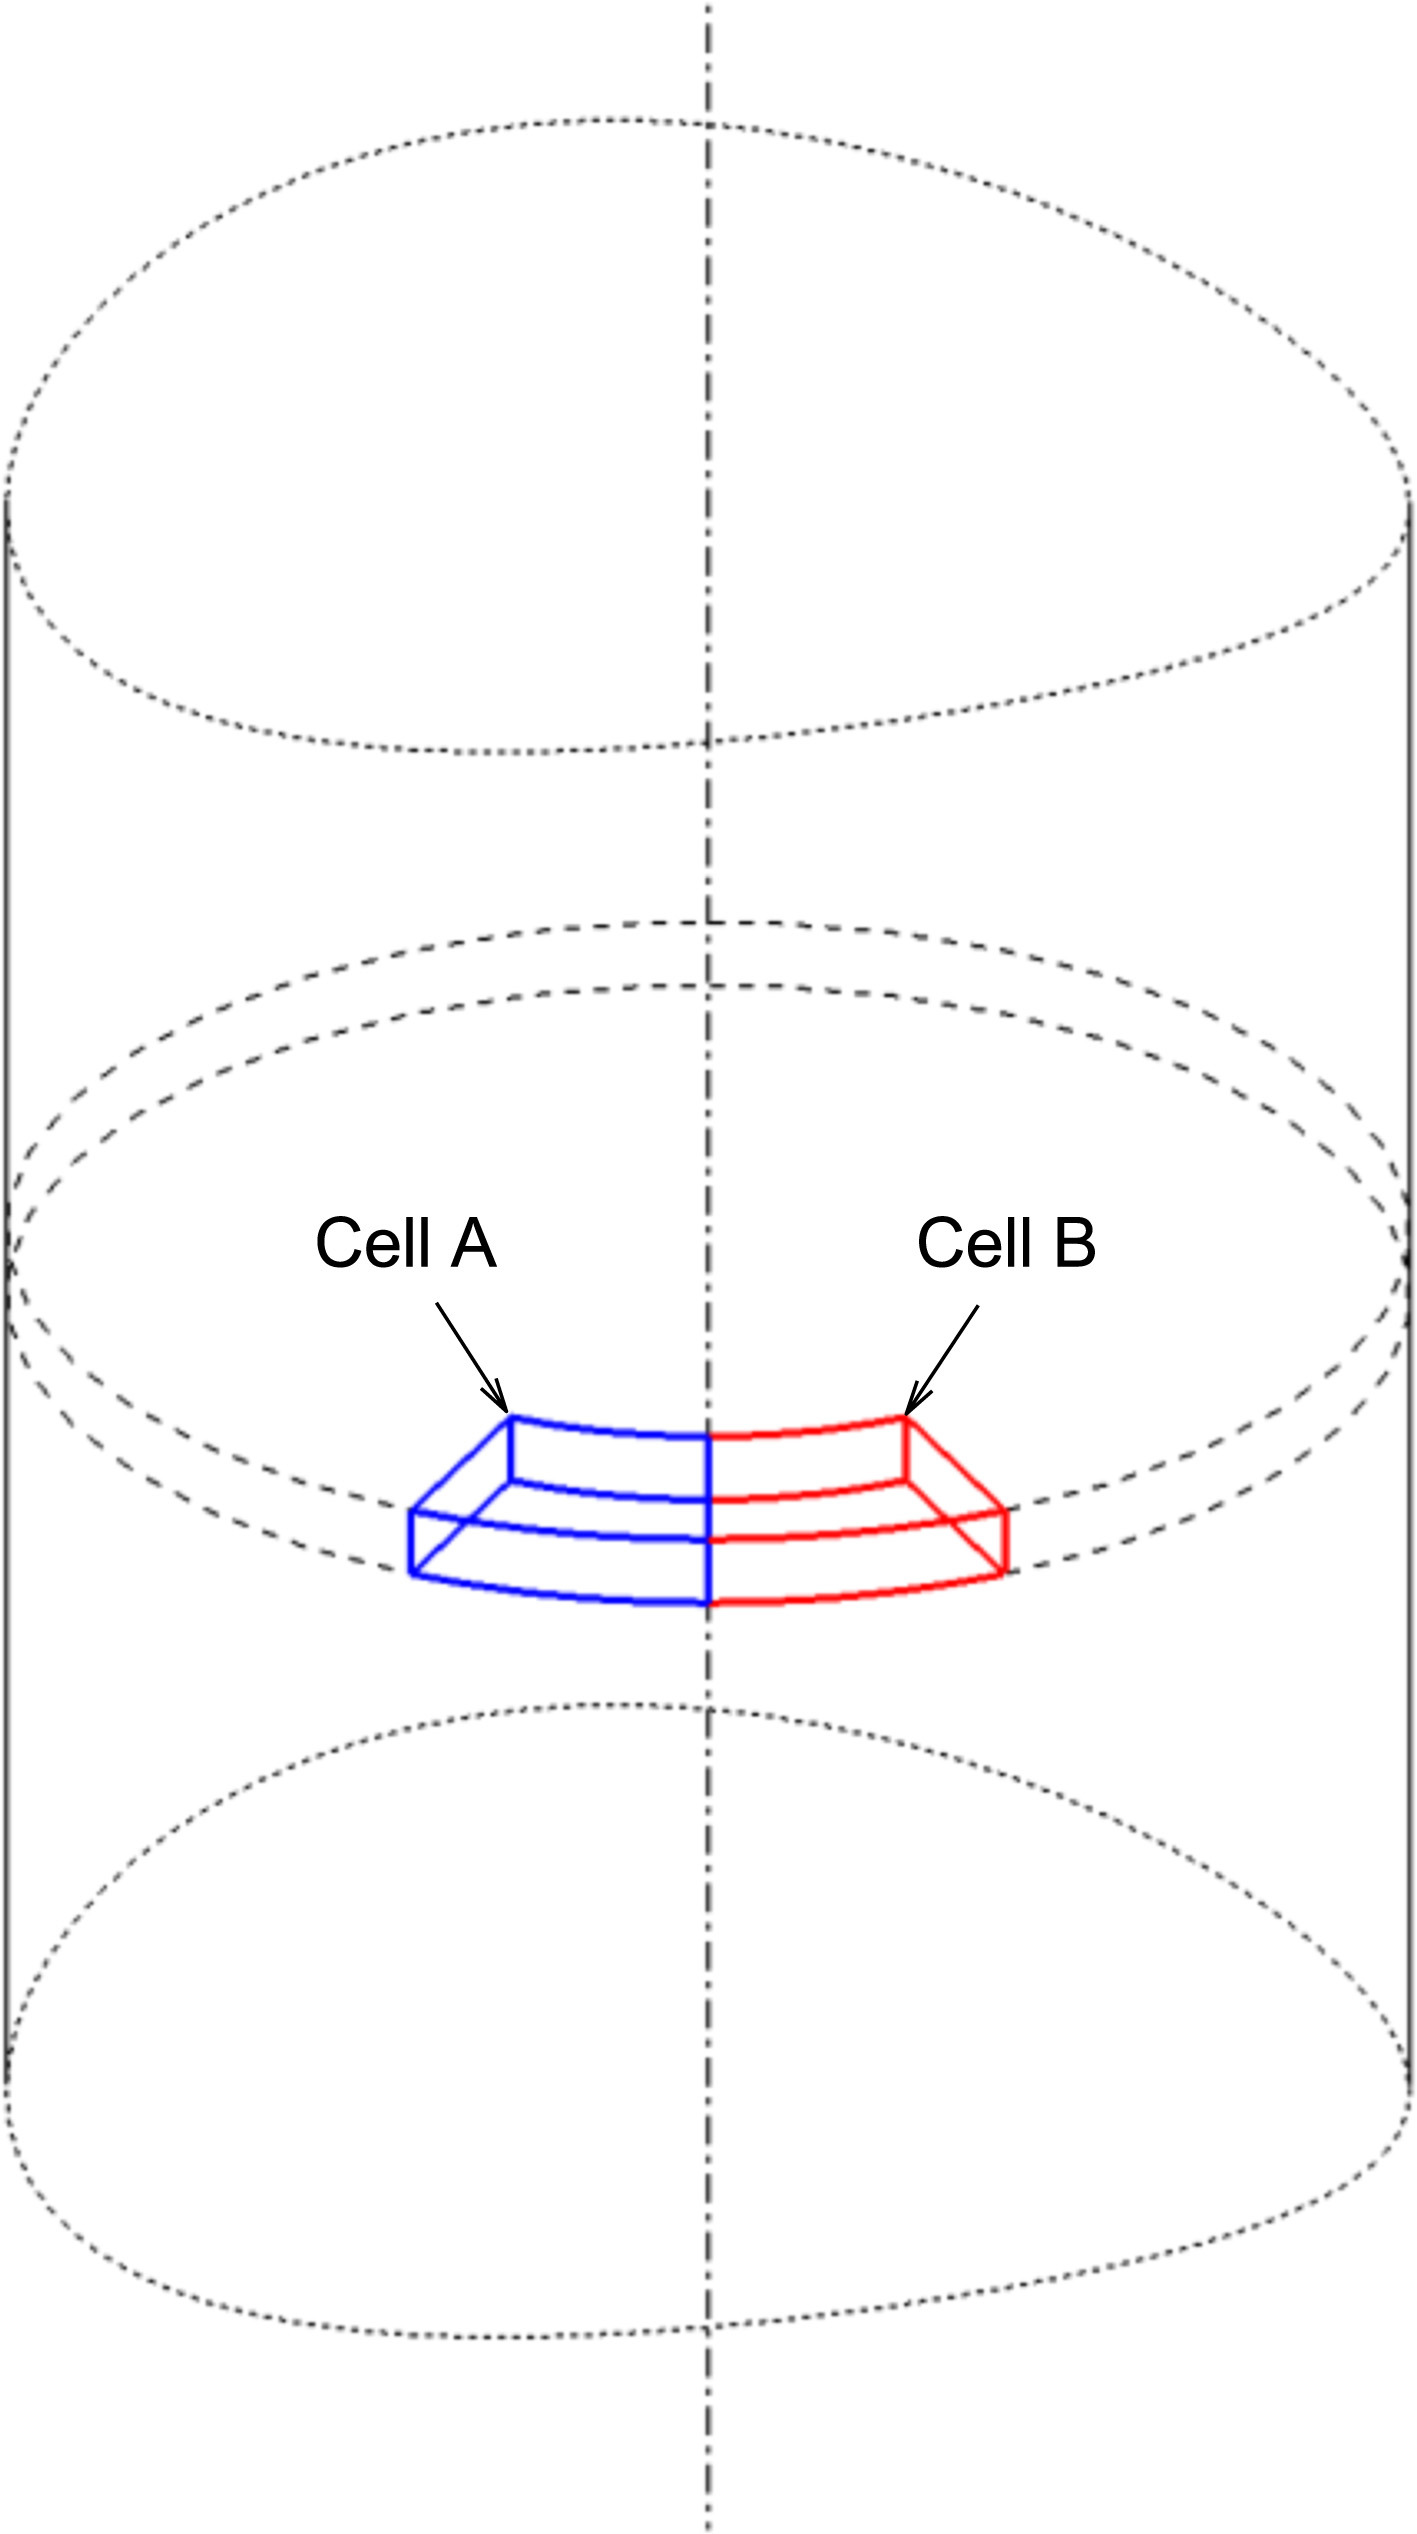
\includegraphics[width=0.575\linewidth]{Figures/rest.jpg}
             \end{figure}
         \end{itemize}
         \columnbreak
         \begin{itemize}
             \item Initialise with last time step
             \begin{figure}
                 \centering
                 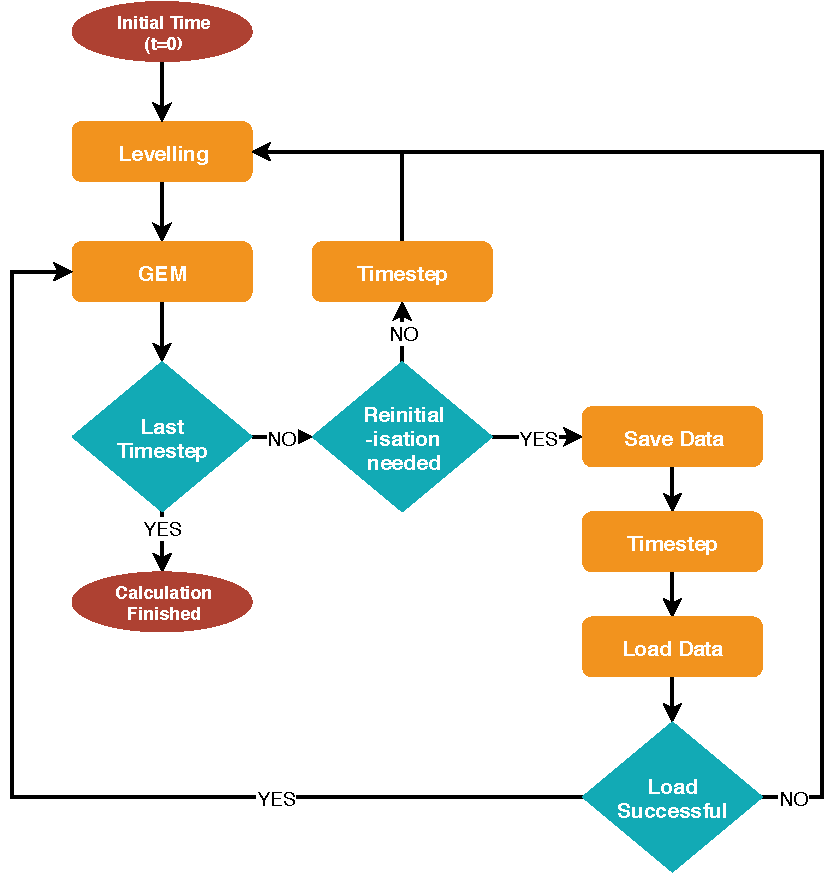
\includegraphics[width=0.925\linewidth]{Figures/Initialisation.pdf}
             \end{figure}
         \end{itemize}
     \end{multicols}
    }

    
     \begin{frame}{Gibbs Energy Minimisation}
         \onslide<1-4>{\begin{itemize}
 	        \item<1->Hessian Solver \[\mtx{H}\cdot\vec{\pi}=\vec{\zeta}\]
 	    \end{itemize}}
\only<2>{\begin{equation*}\label{eq:Hessian_mat}
        \mathbf{H} = 
        \begin{bmatrix}
            r_{j=1,k=1} & \dots & r_{j=1,k=C} & \phi_{j=1,\lambda=1} & \dots & \phi_{j=1,\lambda=\Lambda} & \nu_{j=1,\omega=1} & \dots & \nu_{j=1,\omega=\Omega} \\
            \vdots & \ddots & \vdots & \vdots & \ddots & \vdots & \vdots & \ddots & \vdots \\
            r_{j=C,k=1} & \dots & r_{j=C,k=C} & \phi_{j=C,\lambda=1} & \dots & \phi_{j=C,\lambda=\Lambda} & \nu_{j=C,\omega=1} & \dots & \nu_{j=C,\omega=\Omega} \\
            \phi_{\lambda=1,j=1} & \dots & \phi_{\lambda=1,j=C} & 0 & \dots & 0 & 0 & \dots & 0 \\
            \vdots & \ddots & \vdots & \vdots & \ddots & \vdots & \vdots & \ddots & \vdots \\
            \phi_{\lambda=\Lambda,j=1} & \dots & \phi_{\lambda=\Lambda,j=C} & 0 & \dots & 0 & 0 & \dots & 0 \\
            \nu_{\omega=1,j=1} & \dots & \nu_{\omega=1,j=C} & 0 & \dots & 0 & 0 & \dots & 0 \\
            \vdots & \ddots & \vdots & \vdots & \ddots & \vdots & \vdots & \ddots & \vdots \\
            \nu_{\omega=\Omega,j=1} & \dots & \nu_{\omega=\Omega,j=C} & 0 & \dots & 0 & 0 & \dots & 0 
        \end{bmatrix}
    \end{equation*}}
    
    \only<3>{ \begin{equation*}\label{eq:LagMult_mat}
        \boldsymbol{\pi} = 
        \begin{bmatrix}
            \pi_{j=1}^{m+1} \\
            \vdots \\
            \pi_{j=E}^{m+1} \\
            \pi_{\lambda=1}^{m+1} \\
            \vdots \\
            \pi_{\lambda=\Lambda}^{m+1} \\
            \pi_{\omega=1}^{m+1} \\
            \vdots\\
            \pi_{\omega=\Omega}^{m+1}
        \end{bmatrix}
    \end{equation*}}
    
    \only<4>{ \begin{equation*}\label{eq:Constraint_mat}
        \boldsymbol{\zeta} = 
        \begin{bmatrix}
            b_{j=1} +  \sum_{\lambda=1}^{\Lambda} \sum_{i=1}^{N_\lambda} \left( \frac{\mu_{i(\lambda)}^{m}}{RT} -1 \right)n_{i(\lambda)}^{m} \nu_{i,j=1}\\
            \vdots \\
            b_{j=E} +  \sum_{\lambda=1}^{\Lambda} \sum_{i=1}^{N_\lambda} \left( \frac{\mu_{i(\lambda)}^{m}}{RT} -1 \right)n_{i(\lambda)}^{m} \nu_{i,j=E}\\
            \sum_{i=1}^{N_{\lambda=1}} \left( \frac{\mu_{i(\lambda=1)}^{m}}{RT} -1 \right)n_{i(\lambda=1)}^{m} \\
            \vdots \\
            \sum_{i=1}^{N_{\lambda=\Lambda}} \left( \frac{\mu_{i(\lambda=\Lambda)}^{m}}{RT} -1 \right)n_{i(\lambda=\Lambda)}^{m} \\
            \frac{\mu_{\omega=1}^{m}}{RT} \\
            \vdots\\
            \frac{\mu_{\omega=\Omega}^{m}}{RT} \\
        \end{bmatrix}
    \end{equation*}
}
     \end{frame}
    
     \begin{frame}{Gibbs Energy Minimisation}
         \begin{itemize}
 	        \item Phase assemblage algorithm
 	    \end{itemize}
 	    \begin{figure}
 	        \centering
 	        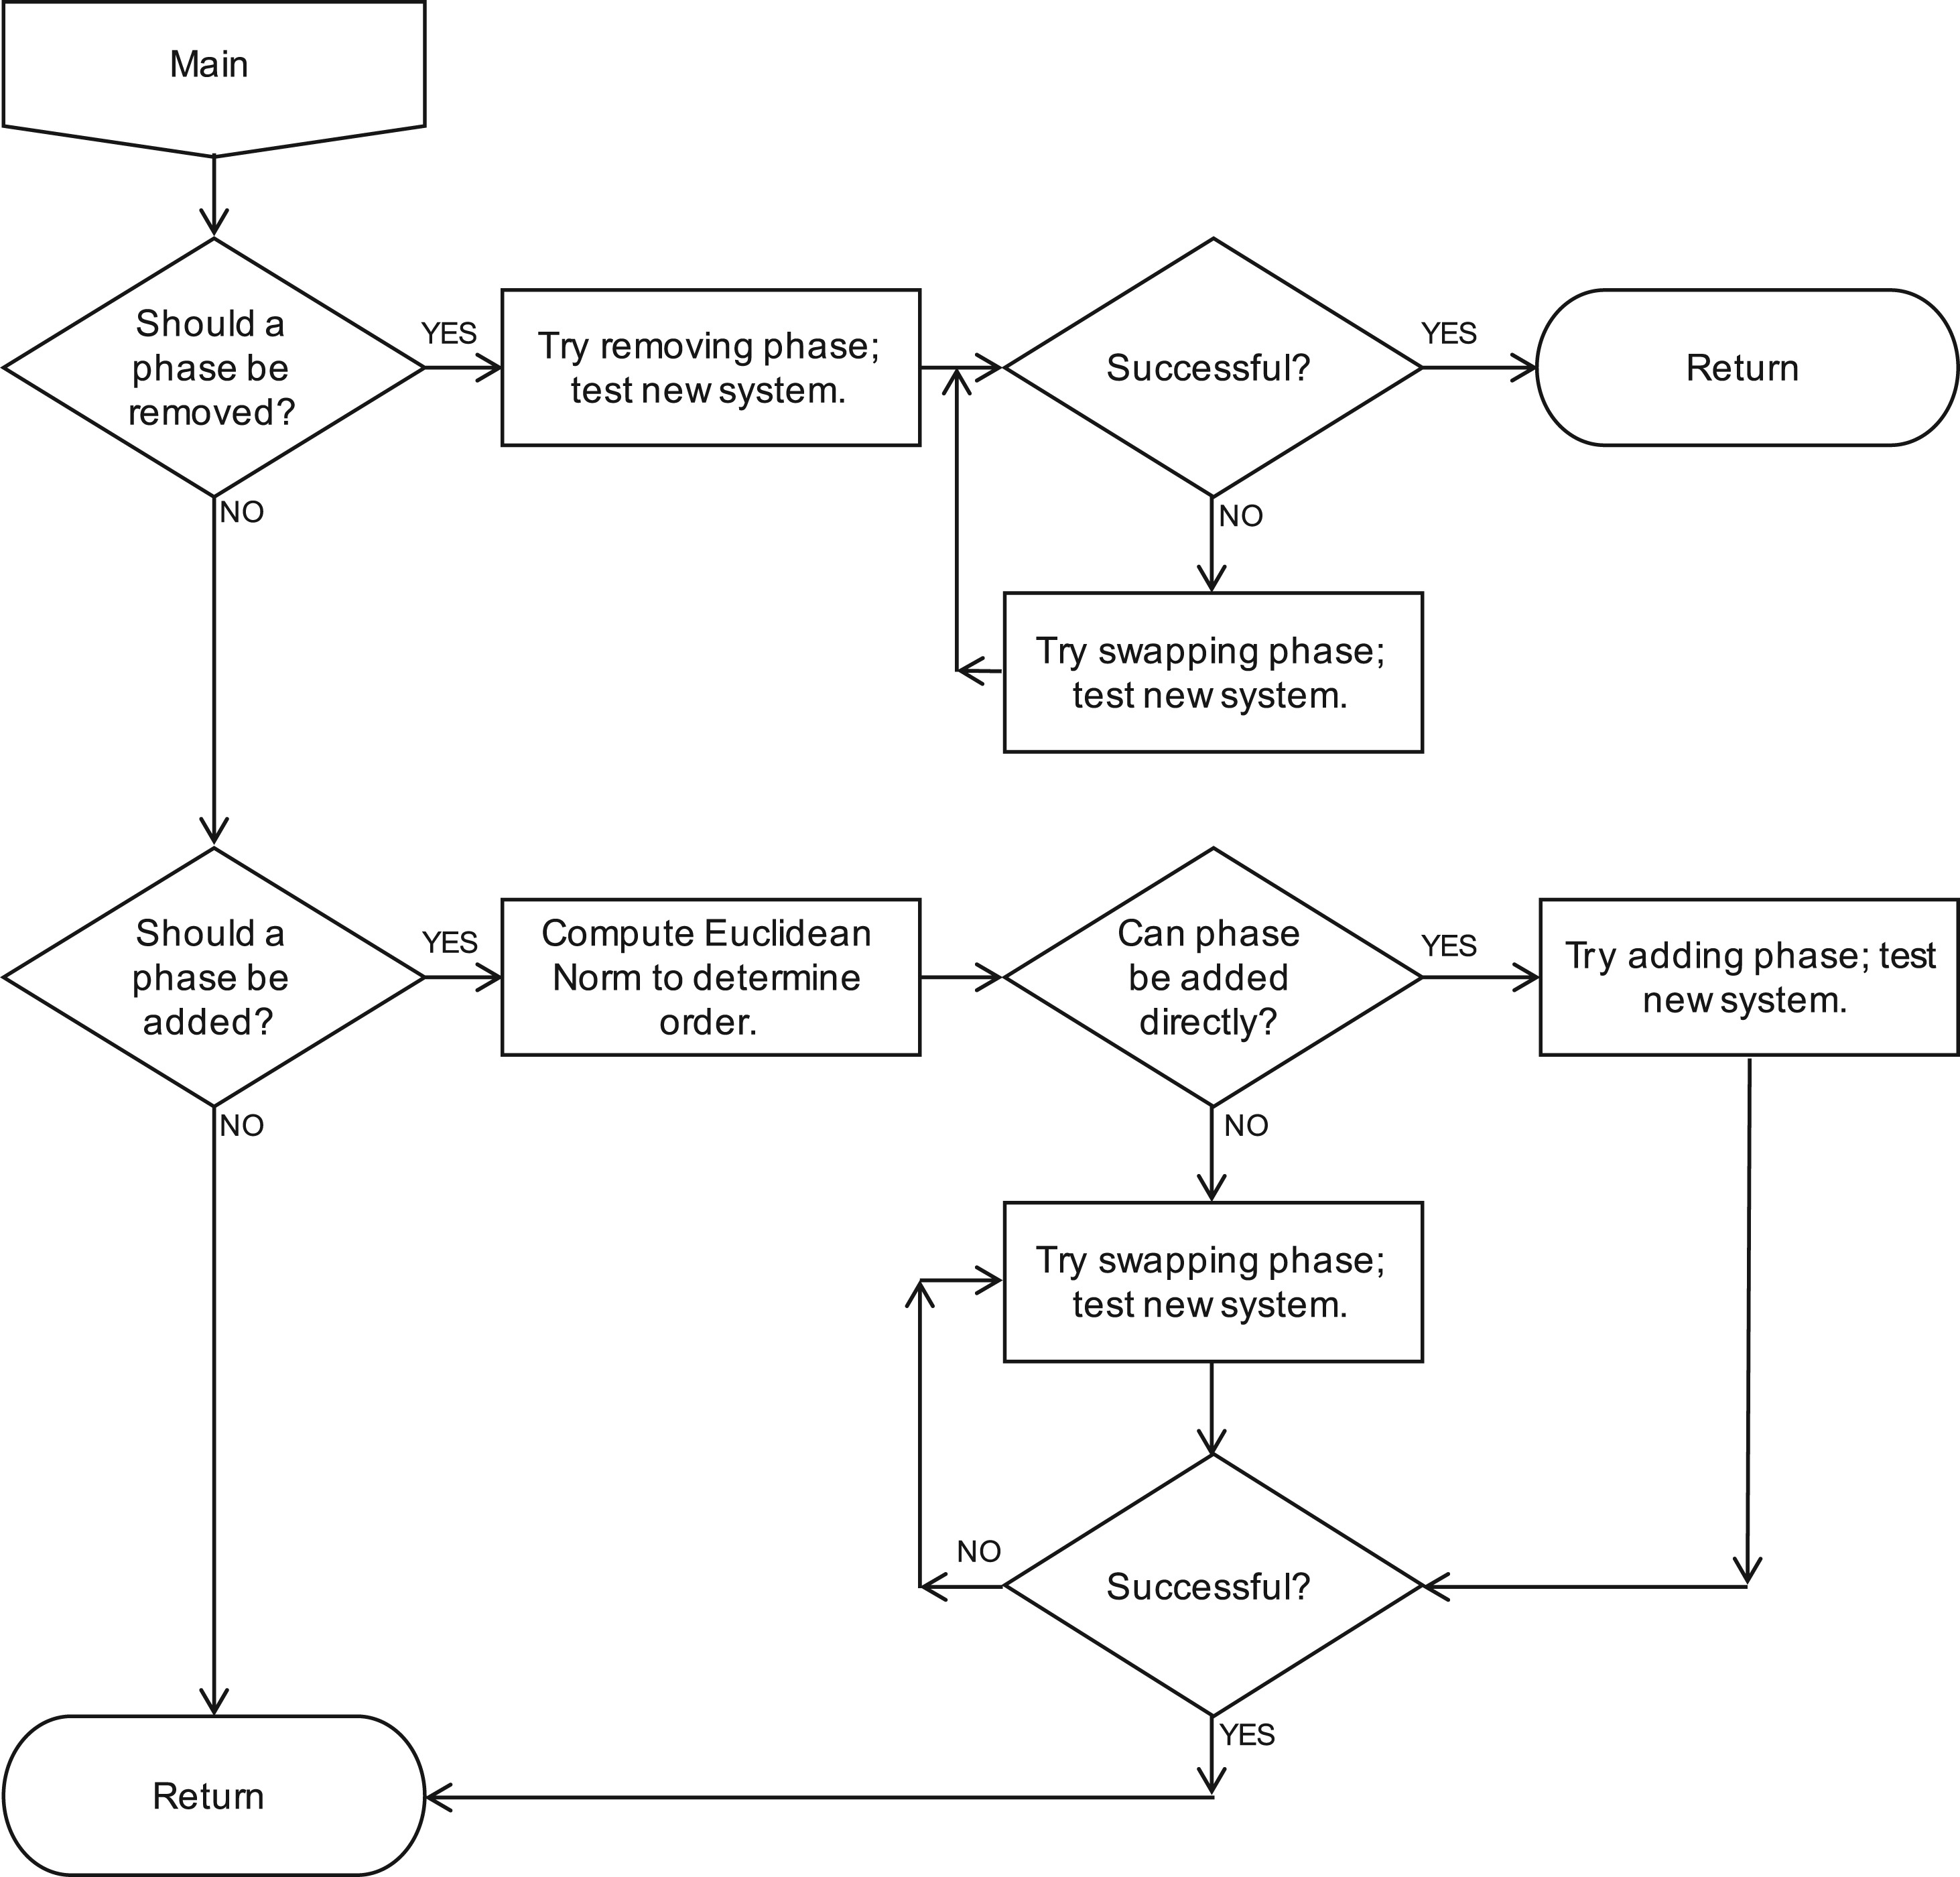
\includegraphics[width=0.45\linewidth]{Figures/Phase_assemblage.jpg}
 	    \end{figure}
     \end{frame}
    
     \begin{frame}{Gibbs Energy Minimisation}
         \begin{itemize}
 	        \item Line Search algorithms
 	   % \end{itemize}
 	    \begin{figure}
 	        \centering
 	        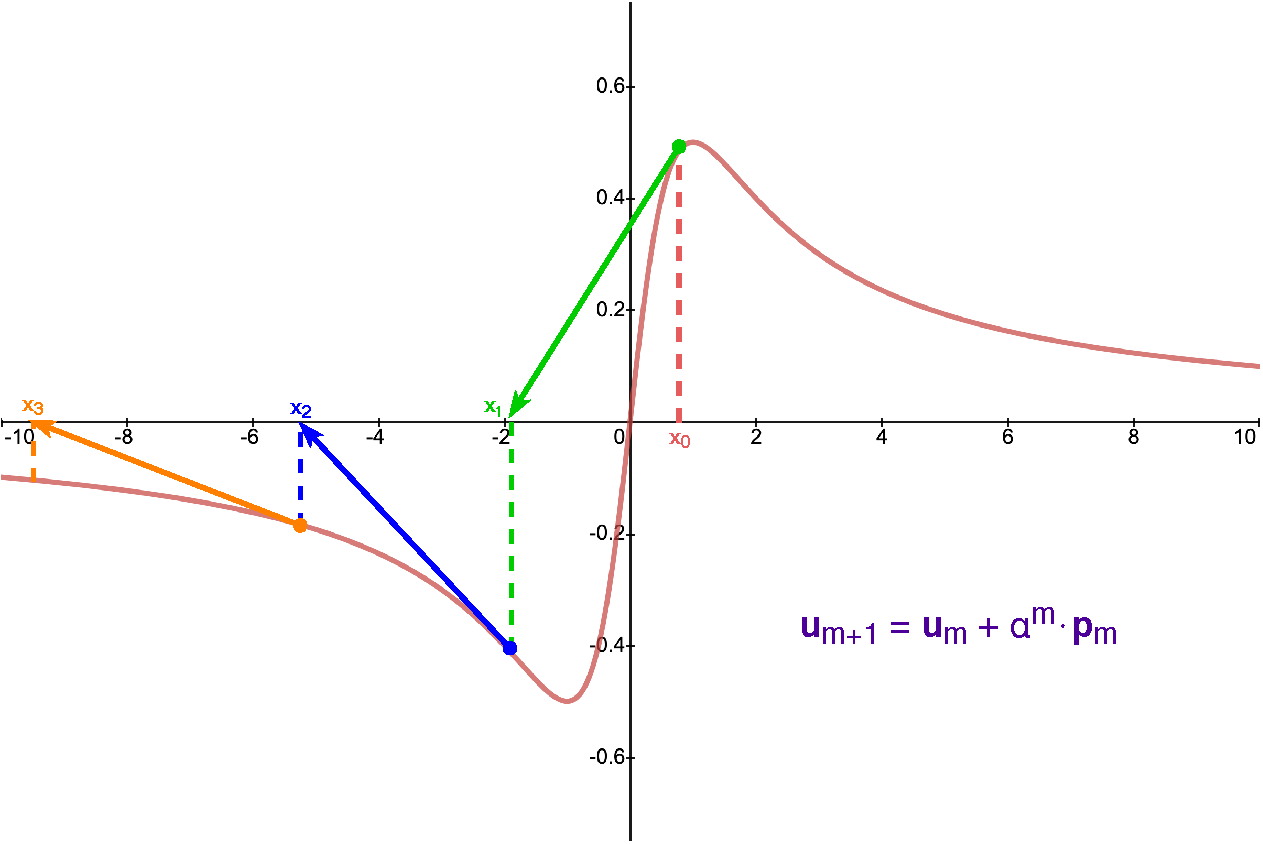
\includegraphics[width=0.5\paperwidth]{Figures/Line_search.pdf}
 	    \end{figure}
 	   % \begin{itemize}
 	        \item Use of Wolfe/Armijo conditions can help avoid divergence.
 	    \end{itemize}
     \end{frame}
    
     \begin{frame}{Global Optimisation}
         \begin{itemize}
             \item The Gibbs energy function of non-ideal phases may be non-convex, yielding multiple local minima. This makes finding global minimum a challenge.
         \end{itemize}
         \begin{figure}
             \centering
             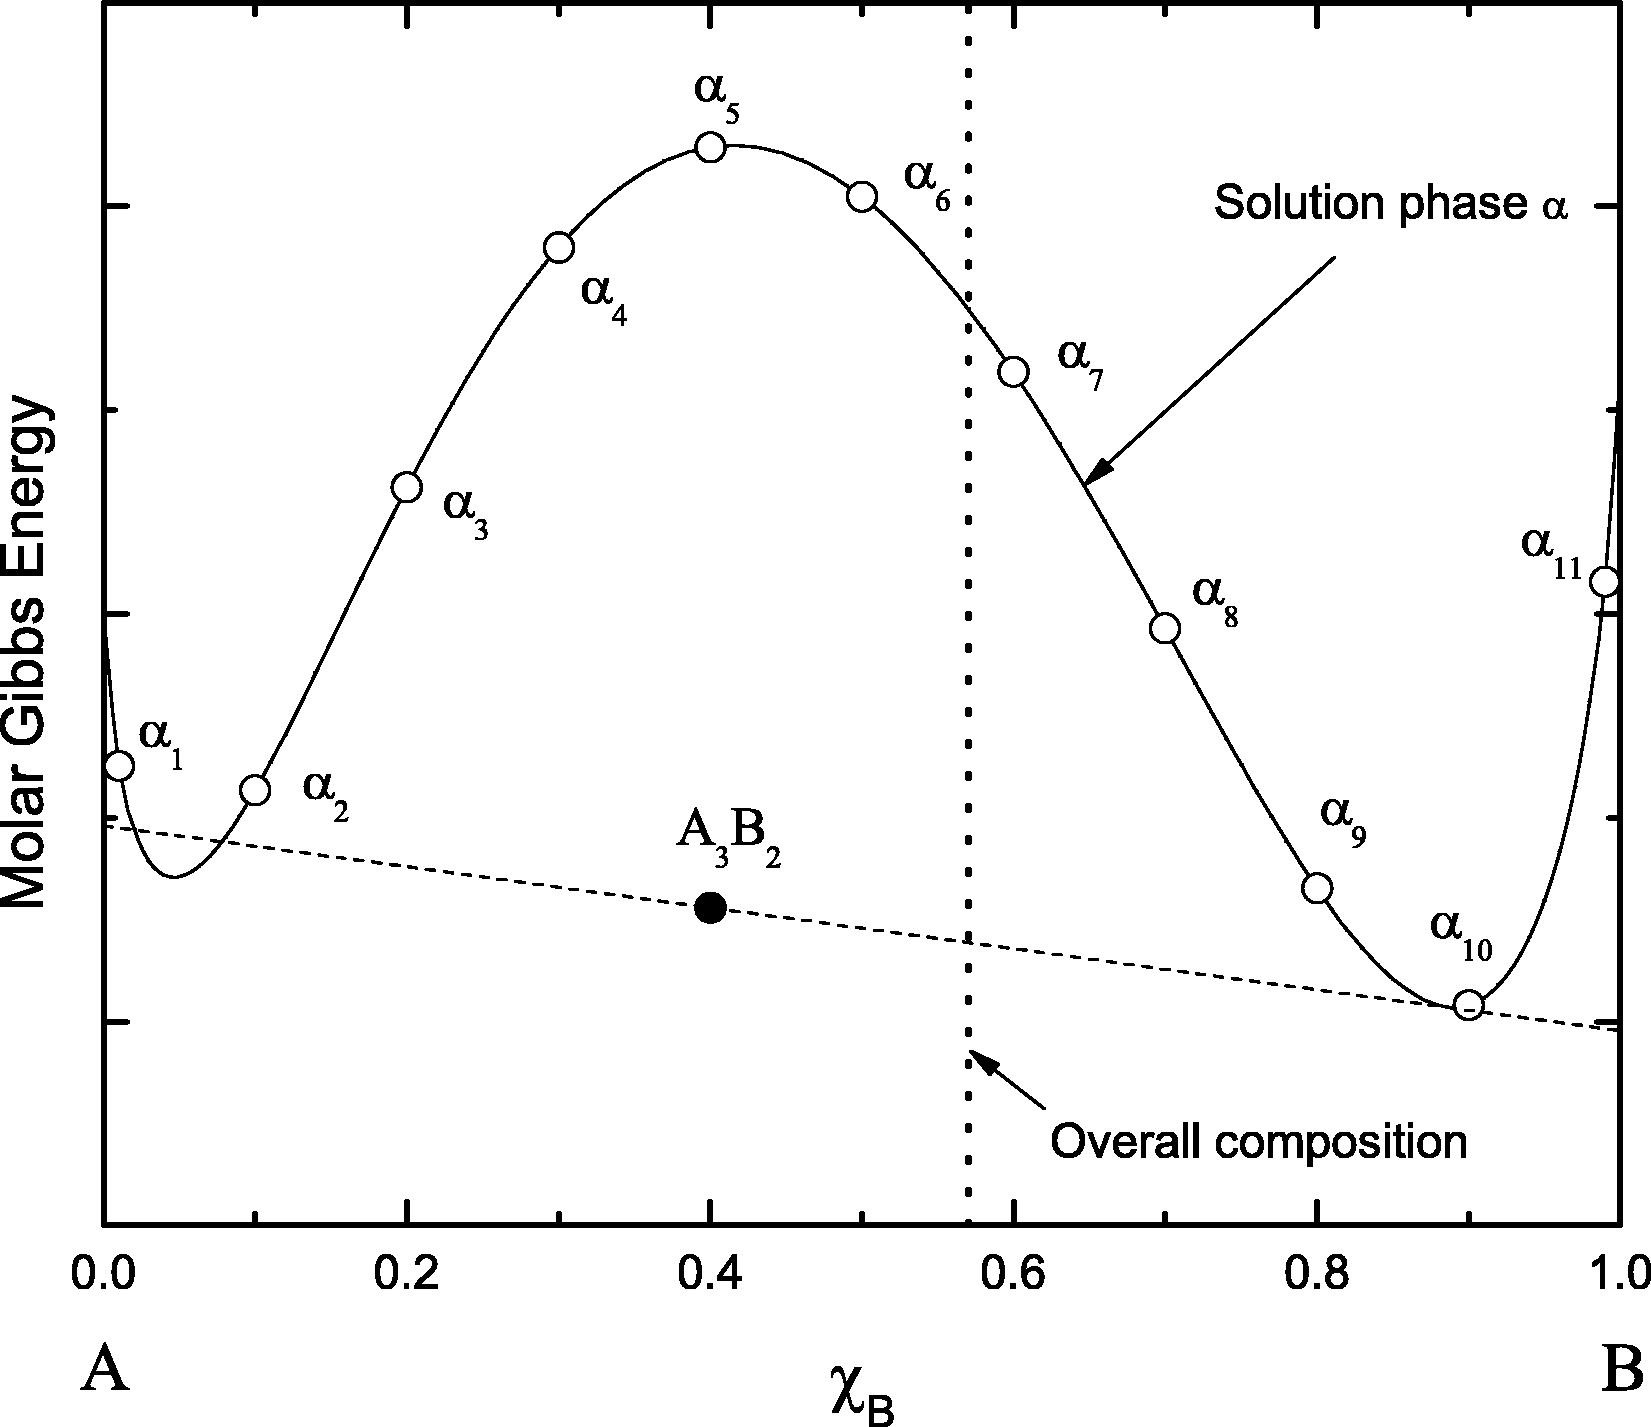
\includegraphics[width=0.5\linewidth]{Figures/Global_opt1}
         \end{figure}
     \end{frame}
    
      \begin{frame}{Global Optimisation}
         \begin{itemize}
             \item Mathematically, global optimisation implies finding the Gibbs plane that satisfies the sufficient condition: \[\pi_{\lambda} = \min_{\lambda} \sum_{i=1}^{N_{\lambda}}x_{i({\lambda})} \left (\mu_{i({\lambda})} - \sum_{j=1}^C \nu_{i,j}\Gamma_j \right )\]
             \item No global optimisation technique guarantees the ability of finding a global extremum of a non-convex function.
             \item Searching for a global minimum becomes increasingly more difficult as the size of the system increases.
             \item The computational effort associated with performing this task can increase very rapidly in large systems.
         \end{itemize}
         % \begin{figure}
         %     \centering
         %     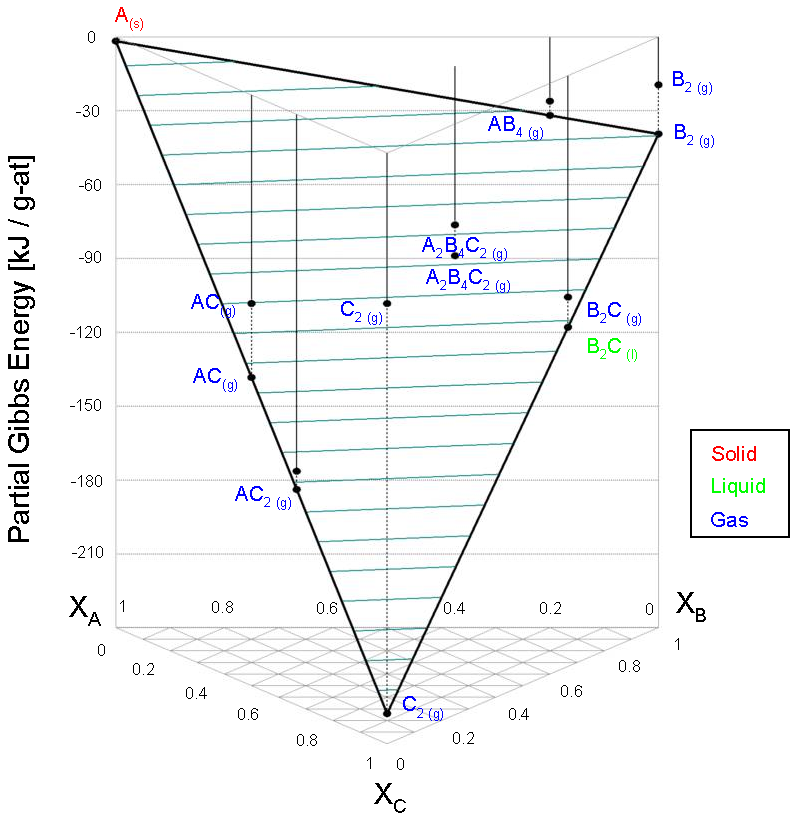
\includegraphics[width=\linewidth]{figures/Gibbs_plane.pdf}
         % \end{figure}
     \end{frame}

     \begin{frame}{Output}
         \begin{itemize}
             \item Outputs after the Gibbs energy minimisation and global optimisation include moles of phases, species mole fraction in each phase, chemical potentials, Gibbs energy, etc.
             \item The chemical potential of various species can be used to find the driving force for other reactions such as corrosion.
             \item These parameters can also be passed to other MOOSE based codes such as {Marmot} and {Bison}.
         \end{itemize}
     \end{frame}